\documentclass[a4paper,12pt]{elsarticle} %,a4paper %[oneside,12pt,notitlepage]
\usepackage{geometry} %[papersize={8.5in,11in}]%[top=2.41cm, bottom=3cm, left=2.41cm, right=2.41cm]
%\geometry{margin=1.5in}
\usepackage{amsmath,amsthm,amssymb}
\usepackage{mathrsfs}
\usepackage{graphicx}
\usepackage{array}
\usepackage{textcomp}
\usepackage{rotating}
\usepackage{xtab}
\usepackage{graphicx}
\usepackage{subcaption}
%\usepackage[authoryear]{natbib}
\bibliographystyle{abbrvnat} % (For authoryear Elsevier citations)
\setcitestyle{authoryear,open={(},close={)}}
\usepackage{titlesec}
\usepackage{url}
\usepackage[font=small,labelfont=bf]{caption}
\usepackage[utf8]{inputenc}
\usepackage{subcaption}
%\usepackage{pdflscape} % put Table on a4
\usepackage{epstopdf} % Use eps now![outdir=./]
\usepackage{siunitx} % Avoid dancing decimals
\sisetup{separate-uncertainty=true} % Make plusminus signs work in Table/tabular
\usepackage{hyperref} % Put toc in the compiled pdf-file
\hypersetup{colorlinks=true,allcolors=blue}
\usepackage{hypcap}
\usepackage{tabularx,ragged2e} % automatic line break in tables
\usepackage{float}% If comment this, figure moves to Page 2
%\usepackage[sectionbib]{chapterbib} %create bib for each chapter
%\usepackage{floatrow}
%\usepackage{blindtext}
%\usepackage{titlesec} % Chapter in one line
%\titleformat{\chapter}[hang]{\normalfont\huge\bfseries}{\chaptertitlename\ \thechapter:}{1em}{}

%% Format settings
\captionsetup[table]{justification=justified,labelsep=none}
\linespread{1.48}
\setlength{\tabcolsep}{3pt}
%\parindent0pt  % set indent to zero, avoid \noindent
%\raggedbottom


% New arguments
\newcommand{\blind}{0} % blinded version, replace "0" with "1" below.

% New commands
%\newfloatcommand{capbtabbox}{table}[][\FBwidth]
\newcommand{\citeapos}[1]{\citeauthor{#1}'s (\citeyear{#1})}
\newcommand{\hypref}[1]{\mbox{(\ref{#1})}}
\renewcommand{\theenumi}{\roman{enumi}}
\newcommand{\E}{\mathop{\mbox{\sf E}}}
\newcommand{\F}[1]{{\mathbb F}}
\newcommand{\IF}{\boldsymbol{1}}
\newcommand{\quantnet}{\hspace*{\fill} \raisebox{-1pt}{\includegraphics[scale=0.05]{Fig/qletlogo}}\,} % Quantnet icon (right-aligned)

\DeclareMathOperator{\sign}{\text{sign}}
\DeclareMathOperator*{\argmin}{arg\,min}
\DeclareMathOperator*{\argmax}{arg\,max}

% mychapter command
\newcommand{\mychapter}[2]{
	\setcounter{chapter}{#1}
	\setcounter{section}{0}
	\chapter*{#2}
	\addcontentsline{toc}{chapter}{#2}
}
\begin{document}

\begin{frontmatter}

\if0\blind{

\title{Phenotypic convergence of cryptocurrencies} % On the speciation of Cryptocurrencies
%\fnref{fn1}
%\fntext[fn1]{Financial support from the Deutsche Forschungsgemeinschaft via International Research Training Group 1792 ''High Dimensional Nonstationary Time Series'', Humboldt-Universität zu Berlin, is gratefully acknowledged.}

%\subtitle{}
\author[1]{Daniel Traian Pele}
\author[2]{Niels Wesselhöfft}
\author[3]{Wolfgang K.\ Härdle}
\address[1]{Department of Statistics and Econometrics, Faculty of Cybernetics, Statistics and Economic Informatics, The Bucharest University of Economic Studies, 010371 Bucharest, Romania, E-mail: danpele@ase.ro}
\address[2]{Humboldt-Universität zu Berlin, IRTG 1792, Spandauer Str. 1, 10178 Berlin, Germany, E-mail: wesselhn@hu-berlin.de}
\address[3]{Humboldt-Universität zu Berlin, IRTG 1792, Spandauer Str. 1, 10178 Berlin, Germany and School of Business, Singapore Management University, 50 Stamford Road, Singapore 178899}

}\fi

\if1\blind
{
\title{Phenotypic convergence of cryptocurrencies}
 %\mbox{}
}\fi

%\date{\svnday.\svnmonth.\svnyear, SVN-revision: \svnrev}
\date{\;}

%\maketitle

\begin{abstract}
\footnotesize{
\noindent In this paper we show that the financial asset class of cryptocurrencies converges to a unique asset class in comparison to stocks, commodities and exchange rates. In biological terms, individual cryptocurrencies respond to similar selection pressures by developing similar characteristics, leading to a phenotypic convergence of cryptocurrencies. In order to retrieve the phenotype of cryptocurrencies, we find the proximal genus and the specific difference (\textit{genus proximum et differentia specifica}) for the daily time series of cryptocurrencies returns, comparing them to classical asset returns. In this sense, the daily time series of asset returns can be characterized by a multidimensional vector with statistical components like volatility, skewness, kurtosis, tail probability, quantiles, conditional tail expectation or fractal dimension. By using dimension reduction techniques (Factor Analysis) and classification models (Binary Logistic Regression, Quadratic Discriminant Analysis, Support Vector Machines) we are able to classify cryptocurrencies as a new asset class with unique features in the tails of the returns distribution. By using expanding window estimation for the factors, we observe a divergent evolution of the cryptocurrencies class, mainly due to the heavy tail behaviour of the respective return distributions. The codes utilized are available via \url{www.quantlet.de.} \\


\noindent{\em Keywords}: cryptocurrency, classification, multivariate analysis, factor models, phenotypic convergence, divergent evolution  \newline %genus proximum, differentia specifica,
\noindent{\em JEL Classification}: C14, C22, C46, C53, G32}
\end{abstract}

\end{frontmatter}


\section*{Introduction}

Cryptocurrencies, served as a new digital asset, have attracted much attention from both investors and academics. Along with this growing popularity, the market capitalization of cryptocurrencies is increasing substantially. Thus, according to a recent report \citep{TransparencyMarketResearch.2018}, the total capitalization for cryptocurrencies market was around US\$574.3 mn in the year 2017 and is expected to reach US\$6702.1 mn by the end of 2025. Most articles focus on Bitcoin as it is considered the first decentralized cryptocurrency, which has the largest capitalization from its beginning till now. An extensive review of the literature regarding the Bitcoin (BTC) can be found in \cite{Corbet.2018}. \hyperref[table:intro_sources]{Table 1} lists the a synthesis of the empirical findings regarding the statistical properties of the cryptocurrencies, compared to classical assets.
 
Given preceding results from the literature, our contribution to the studies dealing with the cryptocurrencies market is mostly empirical, proving the validity of phenotypic convergence in case of cryptocurrencies. In biology, the phenotype of an organism \citep{Mahner.1997} is the set of the organism's observable characteristics (i.e. morphology, developmental processes, biochemical and physiological properties). Phenotypic convergence or convergent evolution can be defined as "the appearance of similar phenotypes in distinct evolutionary lineages" \citep{Washburn.2016}. If the assets universe is regarded as an ecosystem, then we can construct an analogy with the biological concepts. Thus, the phenotype of an asset can be determined by some statistical features of the time series of price or returns. In order to derive the assets phenotype, we are using a genus-differentia approach, allowing to separate the cryptocurrencies universe from the classical assets.

Our approach is quite different from the existing literature, as most of the reviewed paper are using a low-dimensional approach when trying to differentiate cryptocurrencies from classical assets, by using either market risk indicators or long memory indicators. By using a multidimensional approach and taking into account various statistics describing the tail, moment and memory behaviour of the time series of daily log-returns, we find the proximal genus and the specific difference (\textit{genus proximum et differentia specifica}) of the daily time series of cryptocurrencies returns.
\begin{table}[H]
	\tiny{
\caption{: Empirical findings on the cryptocurrencies market}
\label{table:intro_sources}}

\tiny{
\begin{tabularx}{\textwidth}{p{2cm}|p{4cm}|p{1.5cm}|p{6.3cm}|}
\hline \hline
Authors & Assets & Sample & Findings \\
\hline
\cite{AnneHauboDyhrberg.2016} & BTC, USD/EUR, USD/GBP, FTSE index. & 2010-2015, daily data. & BTC can act as a hedge between UK equities and USD. \\
\cite{Dyhrberg.2016} & BTC, Federal funds rate, USD/EUR, USD/GBP, FTSE index, Gold futures, Gold cash. & 2010-2015, daily data. & BTC ranges in between a USD and a Gold. \\
\cite{AurelioF.Bariviera.2017} & BTC, USD/EUR, USD/GBP. & 2011-2017, daily data. 2013-2016, intraday data. & BTC presents large volatility and long-range memory (Hurst exponent higher than 0.5). Standard deviation of BTC is 10 times greater than other currencies. \\
\cite{Baur.2018} & BTC, Federal  funds rate, USD/EUR, USD/GBP, FTSE index, Gold futures, Gold cash. & 2010-2015, daily data. & BTC returns are not a hybrid of Gold and USD  returns. \\
\cite{GuglielmoMariaCaporale.2018} & BTC, LTC, Ripple, Dash & 2013-2017, daily data. & The four cryptocurrencies exhibit persistence (Hurst exponent higher than 0.5), yet the degree of persistence changes over time. \\
\cite{Hardle.2018} & BTC, XRP, LTC, ETH, Gold and S\&P500 & 2016-2018, daily data. & BTC, XRP, LTC, ETH exhibit higher volatility, skewness and kurtosis compared to Gold and S\&P500 daily returns. \\
\cite{Henriques.2018} & BTC and five exchange traded funds (ETFs): US equities (SPY), US bonds (TLT), US real estate (VNQ), Europe and Far East equities (EFA), and Gold (GLD). & 2011-2017, daily data. & BTC can be a substitute for Gold in an investment portfolio, achieving a higher risk adjusted return. \\
\cite{Jiang.2018} & BTC & 2010-2017, daily data. & Long-term memory and high degree of inefficiency ratio  exists in the BTC market.\\
\cite{Klein.2018} & BTC, CRIX index, Gold, Silver, crude oil prices for West Texas Intermediate (WTI), S\&P500 index, MSCI World and MSCI Emerging Markets 50 index. & 2011-2017, daily data. & BTC returns have the highest mean and standard deviation among all assets. \\
\cite{Selmi.2018} & BTC, Gold, Brent crude oil & 2011-2017, daily data. & Both BTC and Gold would serve the roles of a hedge, a safe haven and a diversifier for oil price movements. \\
\cite{Stosic.2018} & Top 119 cryptocurrencies. & 2016-2017, daily data. & Collective behaviour of the cryptocurrency market. \\
\cite{Takaishi.2018} & BTC, GBP/USD & 2014-2016, intraday data & The 1-min return distribution of BTC is fat-tailed, with high kurtosis; BTC time series exhibits multifractality. \\
\cite{Urquhart.2016} & BTC & 2010-2016, daily data. & Hurst statistic indicates strong anti-persistence (values lower than 0.5). \\
\cite{Wei.2018} & 456 different cryptocurrencies. & 2017, daily data. & Lower volatility for liquid cryptocurrencies. Illiquid cryptocurrencies exhibit strong return anti-persistence in the form of a low Hurst exponent. \\
\cite{Zhang.2018} & 70 \% of cryptocurrencies market. & 2013-2018, daily data. & Cryptocurrencies exhibit heavy tails, quickly decaying returns autocorrelations, slowly decaying autocorrelations for absolute returns, strong volatility clustering, leverage effects, long-range dependence, power-law correlation between price and volume. \\
\cite{Borri.2019} & BTC, ETH, LTC, XRP, Gold Bullion, the CBOE volatility index (VIX), the S\&P400 commodity chemicals index, and the S\&P500 index. & 2017-2018, daily data. & Cryptocurrencies exhibit large and volatile return swings, and are riskier than most of the other assets.\\
\hline \hline
\end{tabularx}}
\end{table}

Trough the means of dimensionality reduction techniques (like Factor Analysis) and classification techniques (like Binary Logistic Regression and Support Vector Machines), we prove that most of the variation among cryptocurrencies, stocks, exchanges rates and commodities can be explained by three factors: the tail factor, the moment factor and the memory factor.

Our results add to the findings from literature by showing that the most important factor which differentiates the cryptocurrencies from classical assets is the tail behaviour of the log-returns distribution. This finding is confirmed by the classical factor analysis, performed on a static basis and also by using the expanding window approach, where the assets universe is seen in an evolutionary dynamic. The most important result of our paper is the discovery of a phenotypic convergence of cryptocurrencies, compared to the classical assets. By using an expanding window approach, we are able to show that the cryptocurrencies have a convergent dynamic in relationship to the classical assets and this convergence is driven mainly by the tail behaviour of the log-returns distribution. More, the cryptocurrencies as a species exhibit a divergent evolution in relation to classical assets.  Originated from biology, the concept of divergent evolution refers to the accumulation of differences between related populations, leading to speciation \citep{Rieseberg.2004}. Divergent evolution is typically exhibited when two populations are exposed to different selective factors, driving their adaptation to the environment \citep{Bergstrom.2016}. A related analysis can be found in \cite{ElBahrawy.2017}, where the cryptocurrencies market is seen as an evolutive system, with several characteristics which are preserved over time. According to \cite{ElBahrawy.2017}, the evolution of the cryptocurrencies market has been ruled by "neutral" forces, i.e. no cryptocurrency has shown any strong selective advantage over the other.

The paper is subsequently organized as follows: the first section describes the statistical methodology used, including Factor analysis, Logistic regression, Support vector machines (SVM) and the evolutive divergence. The second section describes the data-set and interprets the results of the classification; the third section describes the phenotypic convergence, while the last section concludes. The codes used to obtain the results in this paper are available via \url{www.quantlet.de}.  %include has clearpage, input not
\section{Methodology}

The methodology used in this paper has four layers: first, we study the statistical properties of the daily log-returns of the selected assets and we estimate the components of a multidimensional vector describing the behaviour of the time series of assets’ daily log-returns. Second, we apply data dimension reduction and orthogonalization methods (Factor Analysis – FA,) in order to retain the orthogonal factors which maximizes the explained variance. Third, we employ classification techniques (Binary logistic regression, Discriminant analysis, Support Vector Machine – SVM) to obtain the most influential factors discriminating between the cryptocurrencies and the classical assets. Fourth, we prove the validity of the phenotypic convergence, showing that cryptocurrencies poses specific characteristics allowing them to differentiate over time from the classical assets.
\subsection{Taxonomy variables}

According to Aristotle, the definition of a species consists of genus proximum and differentia specifica \citep{Parry.1991}. In order to properly define cryptocurrencies in terms of their genus proximum and differentia specifica, we need an initial dataset of variables that have the statistical power to differentiate between the cryptocurrencies and the classical assets (stocks, exchange rates and commodities).\\
Before introducing the multidimensional dataset used for taxonomy, we define the following notations:
\begin{itemize}
	\item $n$ – the number of assets in the dataset;
	\item $t$ – the time index, $t \in\{1, \ldots, T\}$, where $T$ is the time of the last record in the dataset;
	\item  $P_{i, t}-$ the closing price for asset $i$ in day $t,$ with $i=1\ldots n$,  $t=1 \ldots T$;
	 \item $R_{i, t}=\log P_{i, t}-\log P_{i, t-1}$ - the daily log-return for asset  $i$ in day $t,$ with $i=1\ldots n$,  $t=1 \ldots T$;
	 \item	$R=\left(R_{i, t}\right)_{i=1 \ldots, T}^{\mathrm{T}} \in M(T, n)$ - the initial matrix of the assets’ daily log-returns;
	 \item	$p$ - the number of variables used for taxonomy.
\end{itemize}

The multidimensional dataset used for taxonomy is the matrix $X_{t}=\left(x_{i t_{t}, k}\right)_{i=1 \ldots n \atop k=1 \ldots p} \in M(n, p)$ , whose components are detailed below, estimated for the time interval [1, $t$], with $t=t_{0} \ldots T$, where $t_{0}=[T / 3]$.\\
First, we took into account the moments of the log-returns distribution, through the following parameters:

\begin{itemize}
\item variance: $\sigma_{i t}^{2}=E\left\{{(R_{i}-\mu_{i,t})}^2\right\}$ ;
 \item skewness:  $Skewness_{i t}=E\left\{{(R_{i}-\mu_{i,t})}^3\right\}/{\sigma}_{i t}^{3}$;
 \item kurtosis: $Kurtosis_{i t} =E\left\{{(R_{i}-\mu_{i,t})}^4\right\}/{\sigma}_{i t}^{4}$.
\end{itemize}

Second, we estimated the following parameters of the $\alpha$-stable distribution, in order to capture some scaling properties:
\begin{itemize}
	\item the tail parameter: \textit{Stable\_${\alpha}_{i t}$};
	\item the scale parameter: \textit{Stable\_${\gamma}_{i t}$}.
\end{itemize}

The $\alpha$-stable parameters were estimated using the empirical characteristic function method, following \cite{Koutrouvelis.1980} and \cite{Koutrouvelis.1981}. For computational efficiency, we used the fast parallel $\alpha$-stable distribution function evaluation and parameter estimation, through the Matlab library \textit{libstable} \citep{JulianMoreno.2017}.\\
Third, we estimated the quantiles and the conditional tail expectations for the distribution of log-returns, in order to capture the tail behaviour:
\begin{itemize}
	\item quantiles: ${Q}_{\alpha ; i t},$ with $\alpha \in\{0.005,0.01,0.025,0.05,0.95,0.975,0.99,0.995\}$;
	\item conditional left tail expectation: $C T E_{\alpha, i t}\left(R_{i t}\right)=E\left[R_{i t} | R_{i t}<Q_{\alpha ; i t}\right]$, for $\alpha \in\{0.005,0.01,0.025,0.05\}$;
	\item conditional right tail expectation: $C T E_{\alpha, i t}\left(R_{i t}\right)=E\left[R_{i t} | R_{i t}>Q_{\alpha ; i t}\right]$, for $\alpha \in\{0.95,0.975,0.99,0.995\}$.
\end{itemize}
From a market risk perspective, the left tail quantiles can be assimilated to Value-at-Risk, the conditional left tail expectation can be regarded as Expected Shortfall, while the conditional right tail expectation can be seen as the Expected Upside.
Fourth, we estimated the following parameters, in order to capture the memory properties:
\begin{itemize}

	\item first order autocorrelation of the time series of daily log-returns: ${\rho}_{i t}(1)$ ;
	\item Hurst exponent: ${H}_{i t}$. The Hurst exponent \citep{Hurst.1951} of the time series of daily log-returns was estimated based on the discrete second-order derivative in the wavelet domain \citep{ISTAS.1997}.
\end{itemize}
Our multidimensional dataset can be seen as a tensor $\mathscr{X} \in \mathrm{R}^{n\times p\times T'}$, where $n$ is the number of assets, $p=23$ is the number of variables and $T'=T-t_0$ is the number of time points.



\subsection{Factor Analysis}

The most popular methods used to synthesize and extract relevant information from large datasets are Principal Components Analysis (PCA) and Factor Analysis (FA)\citep{Bartholomew.2011}. In this paper, we are using Factor Analysis to extract the main factors explaining the variation in the initial dataset, the reason for this being the fact that PCA is a linear combination of variables, while Factor Analysis is a measurement model of a latent variable. The aim of the factor analysis (FA) is to explain the outcome of the $p$ variables in the data matrix $X$ using fewer variables, the so-called factors \citep{Hardle.2012}. The orthogonal factor model is given by:
\begin{align}
X&=QF+U+\mu\\
(p\times 1)&=(p\times k) (k\times 1) + (p\times 1)+(p\times 1),
\end{align}

with the following notations:
\begin{itemize}
  \item $X$ is the initial matrix of $p$ variables.
  \item $F$ are the common $k$ factors $(k<<p)$.
  \item $Q$ is a matrix of the non-random loadings of the common factors $F$.
  \item $U$ is a matrix of the random specific factors.
  \item $\mu$ is the vector of the means of initial $p$ variables.
  \item the random vectors $F$ and $U$ are unobservable and uncorrelated.
\end{itemize}

In our paper, the initial factor pattern is extracted using the principal component method, followed by a VARIMAX rotation to insure orthogonality of the factors. The Factor Analysis was applied on the entire dataset $X_T$, the $p$ initial variables being estimated for the entire time period $[1,\ldots, T]$. The $p$-dimensional dataset $X_T$ was then projected on the $k$-dimensional space defined by the $k$ orthogonal factors, in order to observe a separation of the assets.



\subsection{Assets Classification}
In order to find \textit{genus proximum and differentia specifica} of the cryptocurrencies, we are using several classification techniques, detailed below.
\subsubsection{Binary Logistic Regression}
 The Binary logistic regression model quantifies the performance of each of the orthogonal factors extracted through the Factor Analysis to discriminate between the cryptocurrencies and classical assets. Thus, we are estimating the following family of models:
\begin{align} \label{form:logit}
P(Y_{i}=1)=\frac{\exp(\beta_{0 j}+\beta_{1 j} F_{j i})}{1+\exp(\beta_{0 k}+\beta_{1 j} F_{j i})},
\end{align}

where $Y_{i}=1$ for cryptocurrencies, $Y_{i}=0$ for classical assets, and $F_j, j\in\left\{1,\ldots,k\right\}$ are the $k$ orthogonal factors retrieved through the factor analysis. Based on the explanatory power and the significance of the model \ref{form:logit}, we can derive the most important factors contributing to the \textit{differentia specifica} of cryptocurrencies.
As a performance measure for the model \ref{form:logit}, we are using $\tilde{R^2}$ \citep{NAGELKERKE.1991}, where:
\begin{align} \label{form:pseudoR}
\tilde{R}^{2}=\frac{1-\left\{\frac{L(\mathbf{0})}{L(\widehat{\boldsymbol{\beta}})}\right\}^{\frac{2}{n}}}{1-\{L(\mathbf{0})\}^{\frac{2}{n}}}.
\end{align}
In formula \ref{form:pseudoR},  $L(0)$ is the likelihood of the intercept-only model, while  $L(\widehat{\boldsymbol{\beta}})$ is the likelihood of the full model.



\subsubsection{Discriminant Analysis}
The aim of discriminant analysis is to classify one or more observations into \textit{a priori} known groups, minimising the error of misclassification \citep{Hardle.2012}.
Formally, Linear Discriminant Analysis (LDA) assumes that the input dataset is multivariate Normal: $X_i\sim N(\mu_i,\Sigma_i)$, where $X_i$ belong to class $\omega_i,\ \Sigma_i=\Sigma_j$. The goal is to project samples $X$ onto a line $Z = w^\top X$, where we select the projection that maximizes the separability. Specifically, we maximize the normalized, squared distance in the means of the classes
  \begin{align}
  w^\ast=\underset{w}{\arg\max}\ \frac{\vert w^\top(\mu_i-\mu_j)\vert^2}{s_i^2+s_j^2},\\
  s_i^2=\sum_{x_i\in\omega_i}(w^\top x_i-w^\top \mu_i)^2=w^\top S_i w,
  \end{align}
  
giving the Linear Discriminant of Fisher \citep{FISHER.1936}:
  \begin{align}
  w^\ast=S_W^{-1}(\mu_i-\mu_j),\ S_W=S_i+S_j.
  \end{align}
Quadratic Discriminant Analysis (QDA) follows the same procedure, but for $X_i\sim N(\mu_i,\Sigma_i)$ belong to the class $\omega_i$, one can relax the condition of equality of covariance matrices by $\Sigma_i\neq\Sigma_j$, allowing for a non-linear classifier.

\subsubsection{Support Vector Machines}

Support Vector Machines (SVM) are a data classification technique, aiming to produce a model which predicts target values based on a set of attributes \citep{Cristianini.2000}. The goal is to find a projection that maximizes margin in a hyperplane of the original data, without any parametric assumptions on the underlying stochastic process. The support vectors are determined via a quadratic optimization problem i.e. given a training data set $D$ with $n$ samples and $2$ dimensions $D=\left(X_{1}, Y_{1}\right), \ldots \left(X_{n}, Y_{n}\right)$, $X_{i} \in \mathbb{R}^{2}, \quad Y_{i} \in[0,1]$, the aim is to  a hyperplane that maximizes the margin
\begin{align}
\min _{w, b} \frac{1}{2}\|w\|^{2},
\text{ s.t.} \quad Y_{i}\left(w^{\top} X_{i}+b\right) \geq 1, i=1, \ldots, n.
\end{align}

\subsubsection{Expanding window modelling}
For observing the assets dynamic, we are using an expanding window approach, allowing to distinguish the evolution of the clusters.
In fact, for $t=t_0,\ldots,T$, where $t_0=[T/3]$, the $p$-dimensional dataset $X_t$ is projected on the $k$-dimensional space defined by the main factors extracted trough the Factor Analysis applied on the dataset $X_T$. By using this projection instead of a time-varying factor model, we are avoiding situations like changes in factors loadings, causing inconsistencies over time. 
\section{Data and Results}

Our dataset is a combination of cryptocurrencies and classical assets (commodities, exchange rates and stocks), covering the time period 10/20/2014 - 10/16/2018 (1006 trading days), for $n=544$ assets (see \hyperref[table:data]{Table 2}).
The reason for choosing this time-span for the analysis is that before 2015 the liquidity in the cryptocurrencies market had been relatively low, the total market capitalization being less than 16 billion US dollars \citep{Feng.2018}.

\begin{table}[H]
\centering
\small{
	\caption{: Dataset}
	\label{table:data}
\begin{tabular}{l S[table-format=-1.2,table-figures-uncertainty=1] l}\hline\hline
\multicolumn{1}{l}{\bfseries Type of Asset}& \multicolumn{1}{c}{\bfseries Number of Assets}& \multicolumn{1}{c}{\bfseries Source}\\ \hline
Cryptocurrencies&14&Coinmarketcap\\
Stocks&497&Bloomberg\\
Exchange rates&13&Bloomberg\\
Commodities&20&Bloomberg\\ \hline\hline
\end{tabular}}
\end{table}

The first component of the dataset contains a representative sample of cryptocurrencies; the cryptocurrencies selected to be part of this analysis are the components of the CRIX Index \citep{Hardle.2018}, sourced from \url{https://coinmarketcap.com/}, for the time interval 10/20/2014 - 10/16/2018. \href{http://thecrix.de/}{The CRyptocurrency IndeX} is a benchmark for the cryptocurrencies market, being realtime computed by the Ladislaus von Bortkiewicz Chair of Statistics at Humboldt University Berlin, Germany. The 15 components of the CRIX index (see the \hyperref[appendix:a]{Appendix A}) account for 90\% of the total cryptocurrencies market capitalization, as seen in \hyperref[fig:figure_1]{Figure 1}. In our analysis, the USDT cryptocurrency was discarded due to the fact that it is an atypical digital currency, having very little variation around the reference value of 1 USD.
\begin{figure}[H]
	\centering
	\includegraphics[width=0.5\textwidth]{Fig/figure_1.png}
	\caption{Cryptocurrencies market capitalization (USD) at 10/19/2018\href{https://github.com/QuantLet/Genus_proximum_cryptos/tree/master/Mkt_Cryptos}{. Mkt\_cryptos.}}
	\label {fig:figure_1}
\end{figure}

The second component of the dataset contains a sample of the most traded commodities indexes, according to Bloomberg (see the \hyperref[appendix:a]{Appendix A}).\\
\indent The third component of the dataset contains a sample of the most liquid exchange rates, according to Bloomberg (see the \hyperref[appendix:a]{Appendix A}).\\
\indent The fourth component of the dataset contains the constituents of the S\&P500 Index, recorded at October 19th 2018. The number of constituents of S\&P500 Index is 505, however in our dataset only 497 of them are listed, i.e. those stock with valid data for the entire time period analysed (the complete list of the stocks included in the analysis can be found in the \hyperref[appendix:a]{Appendix A}).

\subsection{Factor Analysis}

Factor analysis is a classical method used to find latent variables or factors among observed variables, by grouping variables with similar characteristics together. Performing the factor analysis requires, in general, three steps:
\begin{enumerate}
  \item Estimation of the correlation matrix for all the variables, shown in \hyperref[fig:figure_2]{Figure 2}.
  \item Extraction of the factors from the correlation matrix, based on the correlation coefficients of the variables.
  \item Factor rotation, in order to maximize the relationship between the variables and some of the factors.
\end{enumerate}

\begin{figure}[H]
  \begin{minipage}[b]{0.52\textwidth}
\centering
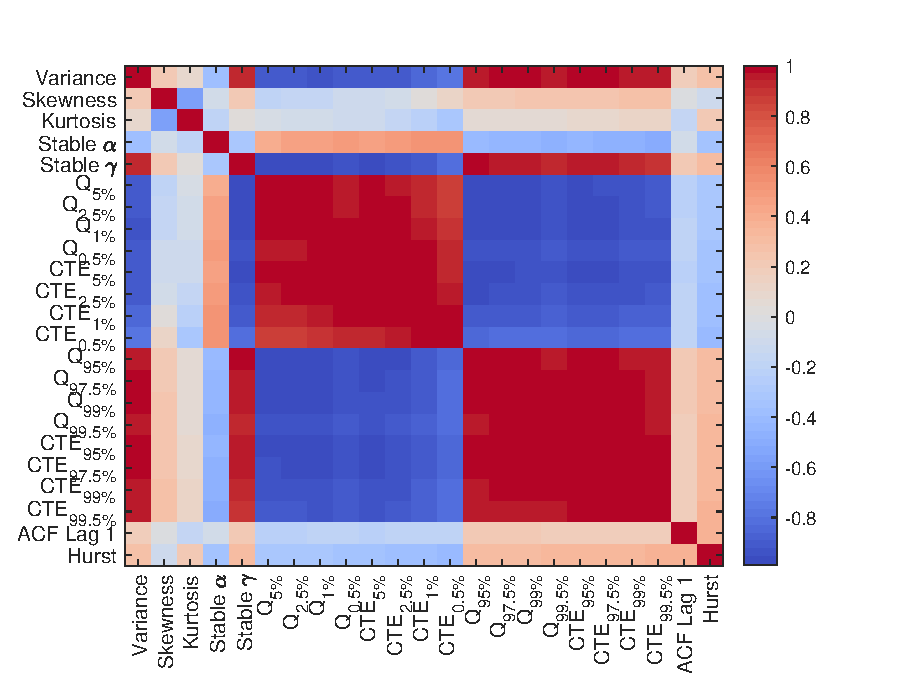
\includegraphics[width=1\textwidth]{Fig/figure_2}
      \caption{Correlation matrix\href{https://github.com/QuantLet/Genus_proximum_cryptos/tree/master/SFA_Cryptos}{. SFA\_cryptos}}
      \label{fig:figure_2}
  \end{minipage}
  \begin{minipage}[b]{0.53\textwidth}
\centering
\includegraphics[width=1\textwidth]{Fig/figure_3}
  \caption{Scree plot\href{https://github.com/QuantLet/Genus_proximum_cryptos/tree/master/SFA_Cryptos}{. SFA\_cryptos}}
    \label{fig:figure_3}
  \end{minipage}
\end{figure}

Based on the eigenvalues criteria, we can select those factors for which the eigenvalue is higher than 1 (see the \hyperref[fig:figure_3]{Figure 3}, where the scree plot is shown). According to this criteria, three factors were selected, accounting for 89.6\% of the total variance.

In order to test the sampling adequacy of the factor analysis, we are using the Kaiser-Meyer-Olkin (KMO); the KMO test should be greater than 0.5 for a satisfactory factor analysis \citep{Tabachnick.op.2013}.\\
The overall KMO test is computed using the following formula:
\begin{align}
KMO=\frac{\sum_{i}\sum_{i\neq j}r_{ij}^2}{\sum_{i}\sum_{i\neq j}r_{ij}^2+\sum_{i}\sum_{i\neq j}u_{ij}^2}
\end{align}
where $R = r_{ij}$ is the correlation matrix and $U = u_{ij}$ is the partial covariance matrix \citep{Cerny.1977, Kaiser.1974}.\\
The individual KMO test is computed using the formula:
\begin{align}
KMO=\frac{\sum_{i\neq j}r_{ij}^2}{\sum_{i\neq j}r_{ij}^2+\sum_{i\neq j}u_{ij}^2}
\end{align}
In fact, the KMO measure represents the proportion of the variance in the input variables that might be caused by underlying factors \citep{Kaiser.1981}. The overall KMO value is $0.903$, pointing out that the factor analysis is suitable for structure detection (see \hyperref[table:table_3]{Table 3}). For the factor rotation, we used the VARIMAX method, which outputs orthogonal factors, also minimizing the number of variables that have high loadings on each factor.\\
\indent{}Based on the rotated factors pattern, the following conclusions can be drawn (see also \hyperref[fig:figure_4]{Figure 4}):
\begin{enumerate}
	\item The first factor – \textbf{the tail factor}, accounting for 76.1\% of the total variance, is highly correlated with the following parameters: the tail parameter alpha and the scale parameter gamma of the stable distribution, the lower and upper quantiles of the distribution of log-returns, the conditional tail expectations and the variance of log-returns.
	\item The second factor – \textbf{the moment factor}, accounting for 8.2\% of the total variance, is highly correlated with the skewness and kurtosis of the distribution of log-returns.
	\item The third factor – \textbf{the memory factor}, accounting for 5.3\% of the total variance, is highly correlated with the Hurst exponent and the first order autocorrelation coefficient of log-returns.
\end{enumerate}

\begin{table}[H]
\centering
\caption{: Kaiser's Measure of Sampling Adequacy}
   \label{table:table_3}
\small{
\begin{tabular}{llll} \hline \hline
Variable & KMO measure & Variable    & KMO measure \\ \hline
$Variance$         & 0.970       &  $Q_{99.5\%}$           & 0.893       \\
$Skewness$         & 0.540       &  $CTE_{0.5\%}$          & 0.877       \\
$Kurtosis$         & 0.510       &   $CTE_{1\%}$          & 0.892       \\
$Stable_\alpha$        & 0.935       &   $CTE_{2.5\%}$          & 0.928       \\
$Stable_\gamma$           & 0.861       &  $CTE_{5\%}$           & 0.884       \\
$Q_{0.5\%}$         & 0.923       &    $CTE_{95\%}$         & 0.878       \\
$Q_{1\%}$         & 0.932       &      $CTE_{97.5\%}$       & 0.898       \\
$Q_{2.5\%}$         & 0.921       &    $CTE_{99\%}$         & 0.884       \\
$Q_{5\%}$         & 0.915       &      $CTE_{99.5\%}$       & 0.874       \\
$Q_{95.5\%}$         & 0.899       &     ${\rho}(1)$        & 0.713       \\
$Q_{97.5\%}$         & 0.948       &     ${H}$        & 0.862       \\
$Q_{99\%}$         & 0.925       & Overall KMO & 0.903       \\ \hline\hline
\end{tabular}}

\end{table}




\begin{figure}[H]
\centering
\includegraphics[width=0.65\textwidth]{Fig/figure_4}
\caption{Loadings of the three factors\href{https://github.com/QuantLet/Genus_proximum_cryptos/tree/master/SFA_Cryptos}{. SFA\_cryptos.}}
   \label{fig:figure_4}
\end{figure}

Based on the factors estimated through the factor analysis, one can map the cryptocurrencies and the classical assets, in order to derive some clustering effect.

\begin{figure}[H]
	\begin{minipage}[b]{0.55\textwidth}
		\centering
		\includegraphics[width=1\textwidth]{Fig/figure_5a}


	\end{minipage}
	\begin{minipage}[b]{0.55\textwidth}
		\centering
		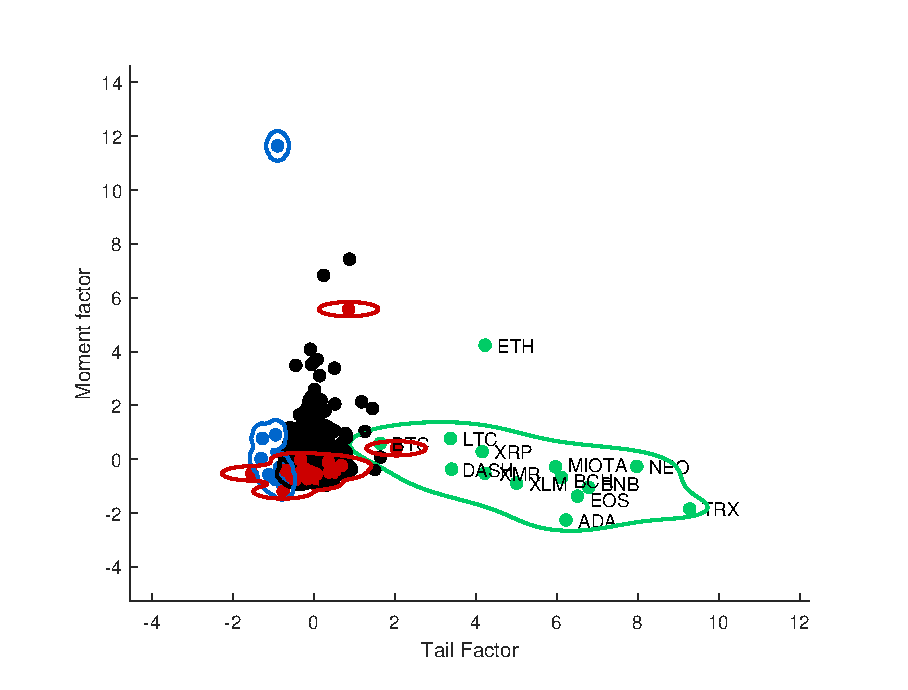
\includegraphics[width=1\textwidth]{Fig/figure_5b}

	\end{minipage}
\caption {Loadings (left) and scores (right) based on tail and moment factor\href{https://github.com/QuantLet/Genus_proximum_cryptos/tree/master/SFA_Cryptos}{. SFA\_cryptos.}}
\label{fig:figure_5}
\end{figure}



Figures 5 to 7 map the cryptocurrencies and the classical assets; the colour code is the following: green - cryptocurrencies, black – stocks, red – commodities, blue – exchange rates. Also, a $95\%$ confidence region is estimated, based on the Bivariate Kernel Density. 
\begin{figure}[H]
	\begin{minipage}[b]{0.55\textwidth}
		\centering
		\includegraphics[width=1\textwidth]{Fig/figure_6a}
		
		
	\end{minipage}
	\begin{minipage}[b]{0.55\textwidth}
		\centering
		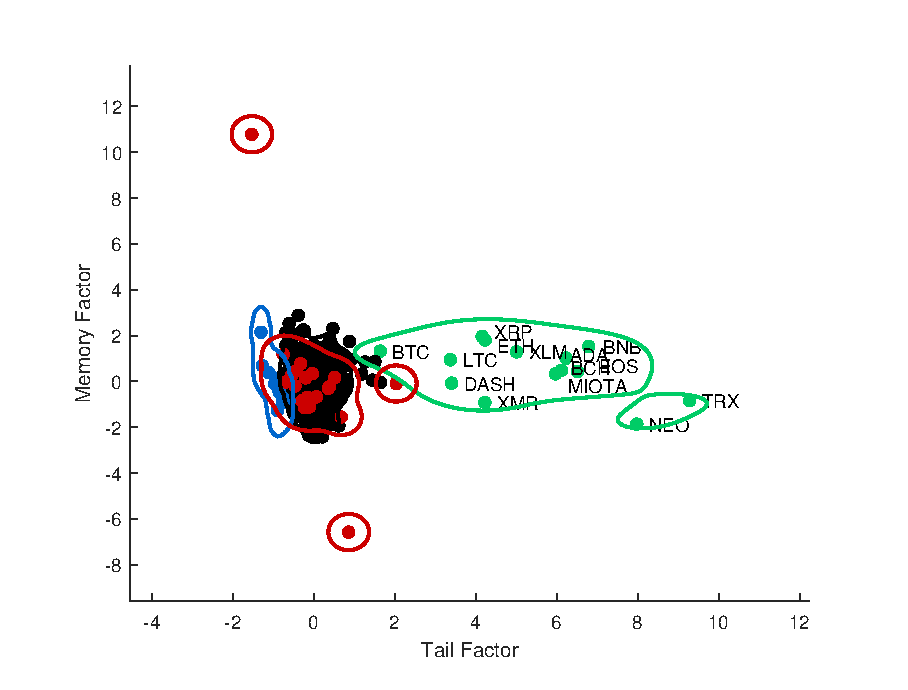
\includegraphics[width=1\textwidth]{Fig/figure_6b}
		
	\end{minipage}
	\caption {Loadings (left) and scores (right) based on tail and memory factor\href{https://github.com/QuantLet/Genus_proximum_cryptos/tree/master/SFA_Cryptos}{. SFA\_cryptos.}}
	\label{fig:figure_6}
\end{figure}

As shown in \hyperref[fig:figure_5]{Figure 5} and \hyperref[fig:figure_6]{Figure 6}, there is a clear separation between cryptocurrencies and classical assets, mainly due to the first factor, the tail factor, while the memory and moment factor are of subliminal subliminal importance (see \hyperref[fig:figure_7]{Figure 7}).
\begin{figure}[H]
	\begin{minipage}[b]{0.55\textwidth}
		\centering
		\includegraphics[width=1\textwidth]{Fig/figure_7a}
		
		
	\end{minipage}
	\begin{minipage}[b]{0.55\textwidth}
		\centering
		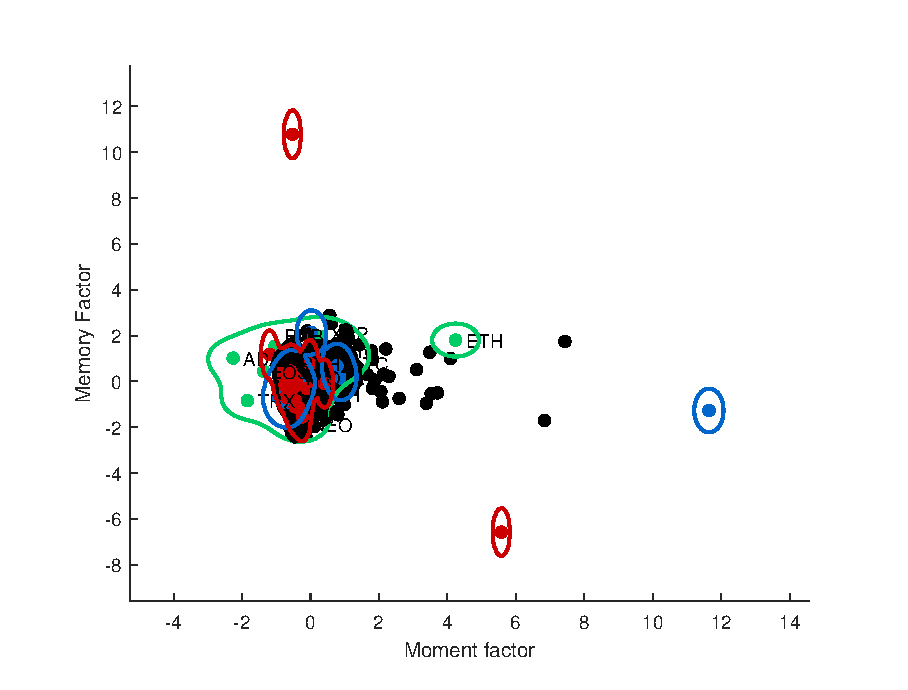
\includegraphics[width=1\textwidth]{Fig/figure_7b}
		
	\end{minipage}
	\caption {Loadings (left) and scores (right) based on moment and memory factor\href{https://github.com/QuantLet/Genus_proximum_cryptos/tree/master/SFA_Cryptos}{. SFA\_cryptos.}}
	\label{fig:figure_7}
\end{figure}

\indent{}Based on the data revealed in the \hyperref[table:table_4]{Table 4}, one can synthesize few characteristics of the cryptocurrencies, that differentiate them from the other assets:
\begin{itemize}
	\item The cryptocurrencies have higher variance of the log-return’s distribution, compared to the classical assets.
	\item The cryptocurrencies exhibit the presence of heavy tails, as indicated by high values of quantiles and conditional tail expectations, i.e. the cryptocurrencies have higher propensity for risk.
	\item The first order autocorrelation is positive in the case of cryptocurrencies, while all the other assets have negative first order autocorrelation, for the analysed time period.
	\item Bitcoin is closer to classical stocks and commodities, in terms of the tail factor, i.e. it’s risk profile can be considered at the border between the classical assets and cryptocurrencies.
\end{itemize}
\begin{table}[H]
	\centering
		\caption{: Assets profile based on the average values of the initial variables}
	\label{table:table_4}
	\small{
		\begin{tabular}{l|l    S[table-format=3.2, round-mode=places,round-precision=3] S[table-format=3.2, round-mode=places,round-precision=3] S[table-format=3.2, round-mode=places,round-precision=3] S[table-format=3.2, round-mode=places,round-precision=3] S[table-format=3.2, round-mode=places,round-precision=3] S[table-format=3.2,round-mode=places,round-precision=3] S[table-format=3.2, round-mode=places,round-precision=3] }\hline\hline
			\multicolumn{1}{l}{\bfseries Factor }&\multicolumn{1}{l}{\bfseries Estimate} &\multicolumn{1}{l}{\bfseries Cryptos}&\multicolumn{1}{l}{\bfseries Stocks} &\multicolumn{1}{l}{\bfseries Commodities} &\multicolumn{1}{l}{\bfseries Exchange Rates}  &\multicolumn{1}{l}{\bfseries Bitcoin}\\ \hline
			
			Tail        & $\sigma^2\cdot10^{3}$                 & 7.88  & 0.28      & 0.37         & 0.03 & 1.50  \\
			factor                 &   $Stable_\alpha$               & 1.436  & 1.703       & 1.753          & 1.759   & 1.319  \\
			&   $Stable_\gamma\cdot10^{3}$          & 36.76  & 8.73       & 9.85           & 3.17   & 16.02  \\
			&   $Q_{0.5\%}$               & -0.255 & -0.056      & -0.052         & -0.015  & -0.139 \\
			&   $Q_{1\%}$               & -0.215 & -0.044      & -0.043         & -0.013  & -0.113 \\
			&   $Q_{2.5\%}$               & -0.148 & -0.032      & -0.034         & -0.01   & -0.086 \\
			&   $Q_{5\%}$               & -0.113 & -0.024      & -0.026         & -0.008  & -0.063 \\
			&   $Q_{95\%}$               & 0.133  & 0.024       & 0.027          & 0.008   & 0.059  \\
			&   $Q_{97.5\%}$               & 0.198  & 0.03        & 0.035          & 0.01    & 0.082  \\
			&   $Q_{99\%}$               & 0.285  & 0.04        & 0.045          & 0.013   & 0.109  \\
			&   $Q_{99.5\%}$               & 0.383  & 0.05        & 0.056          & 0.015   & 0.139  \\
			&   $CTE_{0.5\%}$               & -0.326 & -0.077      & -0.072         & -0.022  & -0.184 \\
			&   $CTE_{1\%}$               & -0.278 & -0.063      & -0.06          & -0.018  & -0.152 \\
			&   $CTE_{2.5\%}$               & -0.217 & -0.048      & -0.046         & -0.014  & -0.123 \\
			&   $CTE_{5\%}$               & -0.172 & -0.038      & -0.038         & -0.011  & -0.098 \\
			&   $CTE_{95\%}$               & 0.233  & 0.035       & 0.04           & 0.011   & 0.092  \\
			&   $CTE_{97.5\%}$               & 0.307  & 0.043       & 0.049          & 0.013   & 0.116  \\
			&   $CTE_{99\%}$               & 0.411  & 0.055       & 0.065          & 0.016   & 0.147  \\
			&   $CTE_{99.5\%}$               & 0.499  & 0.067       & 0.08           & 0.019   & 0.175  \\
			Moment  &     $Skewness$             & 0.973  & -0.508      & 0.285          & -1.223  & -0.283 \\
			factor                 &   $Kurtosis$               & 20.351 & 12.922      & 20.716         & 33.992  & 8.583  \\
			Memory  &     $\rho(1)\cdot10^{3}$             & 40.63  & -2.16      & -13.18         & -11.45  & 16.64  \\
			factor                &    $H$              & 0.567  & 0.509       & 0.533          & 0.514   & 0.565  \\
			
			\hline \hline
	\end{tabular}}

\end{table}




\subsection{Assets classification}

In this section, we list the results of the models presented in Section 2.3, in order to assess the ability of the factors produced through the factor analysis to discriminate between cryptocurrencies and classical assets.\\
First, for each of the three factors we estimated the binary logistic model:
\begin{align} \label{form:logit_est}
P(Y_{i}=1)=\frac{\exp(\beta_{0 j}+\beta_{1 j} F_{j i})}{1+\exp(\beta_{0 k}+\beta_{1 j} F_{j i})},
\end{align}

where $Y_{i}=1$ for cryptocurrencies, $Y_{i}=0$ for classical assets, and $F_j, j\in\left\{1,2,3\right\}$ are the $3$ orthogonal factors retrieved through the factor analysis.

\hyperref[table:table_5]{Table 5} lists the estimated $\beta_{1 j}$ of the binary logistic regression model \ref{form:logit_est}, with the performance measure defined by the equation \ref{form:pseudoR}.

\begin{table}[!ht]
\centering
\small{
\caption{: Estimates of the model \ref{form:logit_est}}
\label{table:table_5}
\begin{tabular}{p{1.5in} p{0.7in} p{0.7in} p{0.7in} } \hline \hline
	\textbf{Exogenous factor} & \textbf{Factor 1} & \textbf{Factor 2} & \textbf{Factor 3} \\ \hline 
	Esimated $\beta_{1}$ & 4.398** & -3.729 & -3.692 \\  
	& (2.086) & (-0.606) & (0.314) \\
	\textit{pseudo-}$R_{adj}^{2} $ & 0.958 & 0.015 & 0.024 \\  
	\hline \hline
\end{tabular}
\\Note: Standard errors in (); ** denotes significance at 95\% confidence level.
\noindent }
\end{table}

As seen in \hyperref[table:table_5]{Table 5}, the most important factor regarding the separation between the cryptocurrencies and the classical assets is the tail factor, while the other two factors have no significant influence.\\
Second, we employed Discriminant Analysis and Support Vector Machines on the space defined by the two first factors (tail and memory).
\hyperref[fig:figure_8]{Figure 8} presents the classification results using Discriminant Analysis. Both linear and quadratic classifiers have a very good classification power, the only cryptocurrency which is misclassified being the Bitcoin (see the \hyperref[table:table_4]{Table 4} for Bitcoin's profile).


\begin{figure}[!ht]
\begin{minipage}[b]{0.48\textwidth}

\centering
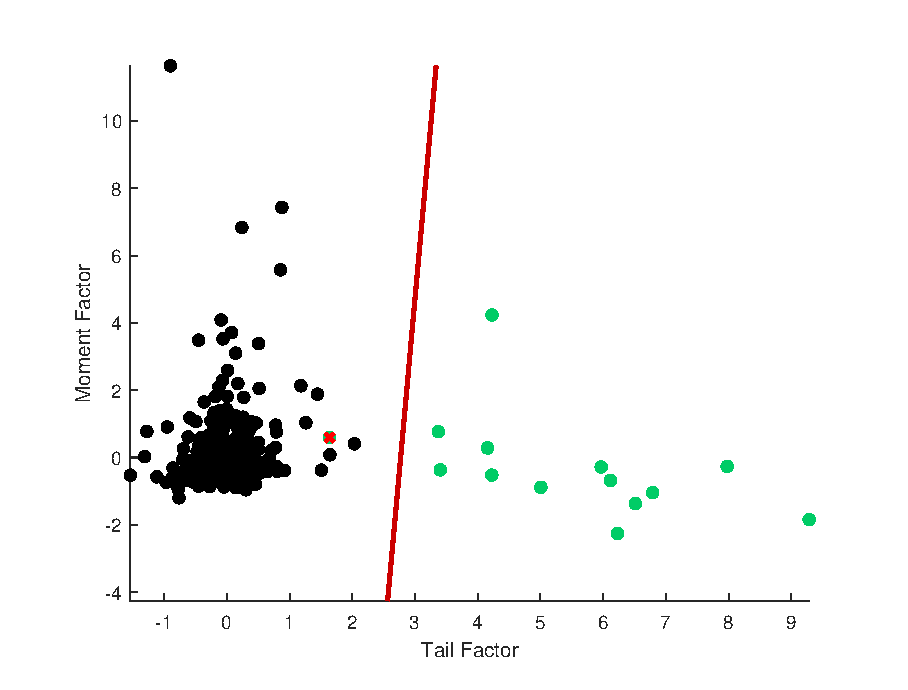
\includegraphics[width=1\textwidth]{Fig/figure_8a}


\end{minipage}
\begin{minipage}[b]{0.48\textwidth}

\centering
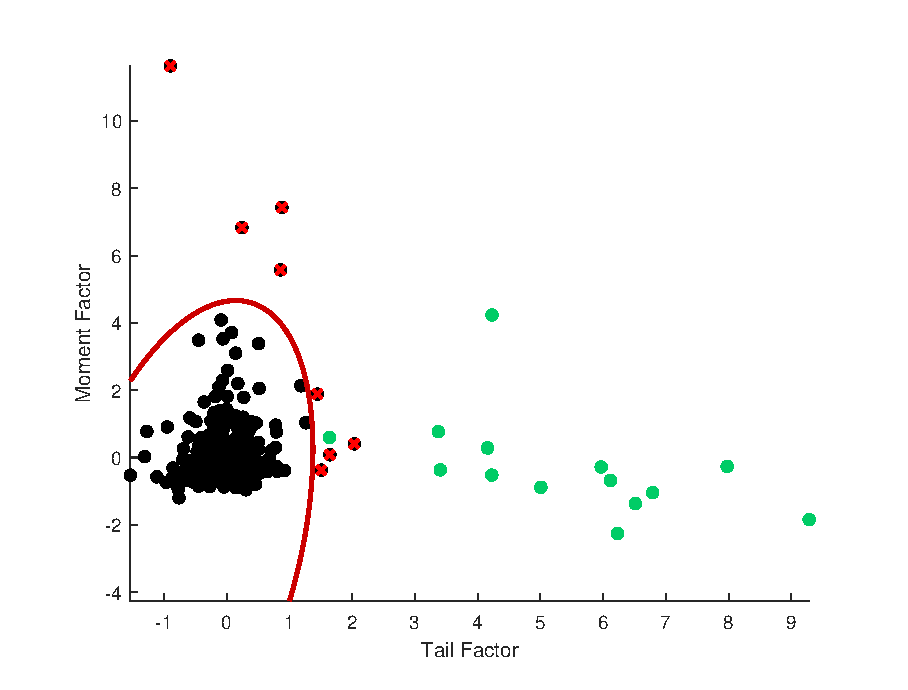
\includegraphics[width=1\textwidth]{Fig/figure_8b}


\end{minipage}
\caption{ Discriminant Analysis: linear(left) and quadratic (right). Green dots denote the cryptocurrencies, while the black dots denote the other assets; the dots highlighted in red are cases of misclassification\href{https://github.com/QuantLet/Genus_proximum_cryptos/tree/master/SFA_Cryptos}{. SFA\_cryptos.}}
	\label{fig:figure_8}
\end{figure}

The same conclusion can be drawn by looking at the results of the Support Vector Machines non-linear classifier, according to which all the cryptocurrencies are correctly classified using the tail factor and the moment factor (see \hyperref[fig:figure_9]{Figure 9}).

\begin{figure}[!ht]
\centering
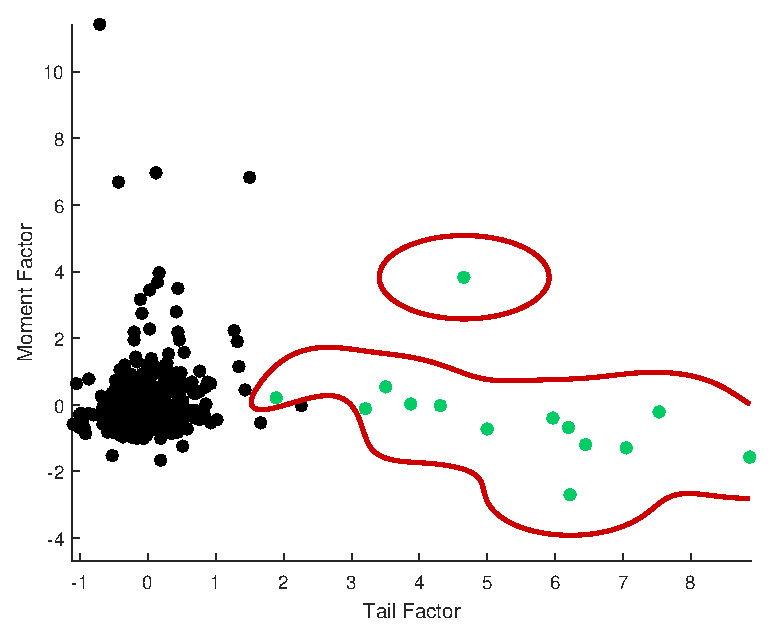
\includegraphics[width=0.48\textwidth]{Fig/figure_9}
\caption{ Support Vector Machines. Green dots denote the cryptocurrencies, while the black dots denote the other assets\href{https://github.com/QuantLet/Genus_proximum_cryptos/tree/master/SFA_Cryptos}{. SFA\_cryptos.}}
	\label{fig:figure_9}
\end{figure}

From an Aristotelian point of view, we can conclude that the differentia specifica of the cryptocurrencies is the tail behaviour of the distribution of daily log-returns.
In other words, based on the tail factor profile, we can conclude that a random asset is likely to be a cryptocurrency if it has the following properties: very long tails of the log-returns distribution (in terms of the left and right quantile and the conditional tail expectation), high variance, high value of the alpha stable scale parameter and value of the alpha stable tail index closer to 1.



\input{3_Evolutive_Divergence/Div}
\section{Conclusions}

In this paper we applied linear Factor models on statistics of log returns in order to discriminate between the cryptocurrencies and traditional assets: stocks, exchange rates and commodities. Utilizing a multidimensional approach, which takes various indicators  into account, which describe the market risk behaviour, tail behaviour and long-memory characteristics of the time series of daily log-returns, we found the proximal genus and the specific difference (genus proximum et differentia specifica) between the daily time series of cryptocurrencies returns and the classical assets returns.\\

Through the means of dimensionality reduction techniques and classification techniques, we showed that large parts of the variation among the cryptocurrencies, stocks, exchanges rates and commodities can be explained by three factors: the tail factor, the moment factor and the memory factor. Our analysis revealed that the main difference between cryptocurrencies and classical assets, in terms of properties of the distribution of daily log-returns, is the tail behaviour, both in the left and in the right tail of the distribution. The moment factor and the memory factor are of subliminal importance for discriminating between cryptocurrencies and classical assets.

Based on the tail factor profile, we can conclude that a random asset is likely to be a cryptocurrency if it has the following properties: very long tails of the log-returns distribution (in terms of the left and right quantile and the conditional tail expectation), high variance, high value of the $\alpha$-stable scale parameter and value of the $\alpha$-stable tail index closer to 1.

From the point of view of the risk analysts and regulators, the non-linear classification techniques applied on the factors extracted provide proficient results in order to discriminate between the cryptocurrencies and the other assets.

The added value of our research is the study of the cryptocurrencies universe using the concepts of phenotypic convergence and divergent evolution. Through the means of an expanding window approach, we are able to depict the evolutionary dynamics of cryptocurrencies universe and show how the clusters formed by projecting the multidimensional dataset on the main factors converge over time.

Viewing the assets universe as a complex ecosystem, we are able to conclude that the cryptocurrencies exhibit both a phenotypic convergence (individual cryptocurrencies develop similar characteristics over time) and a divergent evolution, as different species, compared to the classical assets.

\section*{Acknowledgements}
We would like to thank the editor and the anonymous referees for their valuable comments to this article. Financial support from the Deutsche Forschungsgemeinschaft, Germany via IRTG 1792 ‘‘High Dimensional Non Stationary Time Series’’, Humboldt-Universität zu Berlin, Germany is gratefully acknowledged.


\newcommand{\sectionbreak}{\clearpage}
\appendix
\section*{Appendix A - List of assets used in the analysis}\label{appendix:a}

\begin{table}[H]
	\begin{minipage}[b]{0.48\textwidth}
		\centering
		\tiny{	\caption*{Table A.1: List of commodities}
			\begin{tabular}{llll} \hline\hline
				Nr.crt. & Commodity & Symbol   \\ \hline
				1 & WTI Crude oil & USCRWTIC Index   \\
				2 & Natural Gas & NGUSHHUB Index   \\
				3 & Brent oil & EUCRBRDT Index  \\
				4 & Unleaded Gasoline & RBOB87PM Index   \\
				5 & ULS Diesel & DIEINULP Index  \\
				6 & Live cattle & SPGSLC Index   \\
				7 & Lean hogs & HOGSNATL Index   \\
				8 & Wheat & WEATTKHR Index   \\
				9 & Corn & CRNUSPOT Index   \\
				10 & Soybeans & SOYBCH1Y Index   \\
				11 & Aluminum & LMAHDY Comdty   \\
				12 & Copper & LMCADY Comdty   \\
				13 & Zinc & ZSDY Comdty   \\
				14 & Nickel & CKEL Comdty   \\
				15 & Tin & JMC1DLTS Index   \\
				16 & Gold & XAU Curncy   \\
				17 & Silver & XAG Curncy   \\
				18 & Platinum & XPT Curncy   \\
				19 & Cotton & COTNMAVG Index   \\
				20 & Cocoa & MLCXCCSP Index \\ \hline\hline
		\end{tabular}}
	
	\end{minipage}
	\hfill
	\begin{minipage}[b]{0.48\textwidth}
		\tiny{	\caption*{Table A.2: List of exchange rates}
			\begin{tabular}{llll} \hline \hline
				Nr. crt. & Symbol & Denomination & Name \\ \hline
				1 & EUR & EUR/USD & Euro \\
				2 & JPY & JPY/USD & Japanese Yen \\
				3 & GBP & GBP/USD & Great Britain Pound \\
				4 & CAD & CAD/USD & Canada Dollar \\
				5 & AUD & AUD/USD & Australia Dollar \\
				6 & NZD & NZD/USD & New Zealand Dollar \\
				7 & CHF & CHF/USD & Swiss Franc \\
				8 & DKK & DKK/USD & Danish Krone \\
				9 & NOK & NOK/USD & Norwegian Krone \\
				10 & SEK & SEK/USD & Swedish Krone \\
				11 & CNY & CNY/USD & Chinese Yuan Renminbi \\
				12 & HKD & HKD/USD & Hong Kong Dollar \\
				13 & INR & INR/USD & Indian Rupee \\ \hline \hline
		\end{tabular}}
	
	\end{minipage}
\end{table}

\begin{table}[H]
	\centering
	\tiny{	\caption*{Table A.3: CRIX components at 10/19/2018}
		\begin{tabular}{llll} \hline\hline
			Coin & Symbol & Name & Market Cap (in \$K) \\ \hline
			1 & BTC & Bitcoin & 114,953,322 \\
			2 & ETH & Ethereum & 21,665,771 \\
			3 & XRP & Ripple & 19,035,356 \\
			4 & BCH & Bitcoin Cash & 7,975,384 \\
			5 & EOS & EOS & 5,005,087 \\
			6 & XLM & Stellar & 4,633,717 \\
			7 & LTC & Litecoin & 3,218,216 \\
			8 & USDT & Tether & 2,755,619 \\
			9 & ADA & Cardano & 2,450,912 \\
			10 & XMR & Monero & 1,788,084 \\
			11 & TRX & TRON & 1,624,929 \\
			12 & BNB & Binance Coin & 1,461,507 \\
			13 & MIOTA & Iota & 1,448,470 \\
			14 & DASH & Dash & 1,368,564 \\
			15 & NEO & Neo & 1,108,333 \\ \hline\hline
	\end{tabular}}

\end{table}


The components of the S\&P500 used in the analysis and the entire list of assets can be found \href{https://github.com/QuantLet/Genus_proximum_cryptos/blob/master/list.xlsx}{here}. 

%%%%%%%

\bibliography{references}
\bibliographystyle{elsarticle-harv}%{unsrtnat}

\end{document} 